\begin{figure}[H]

\centering
\subfigure[30Music]
{
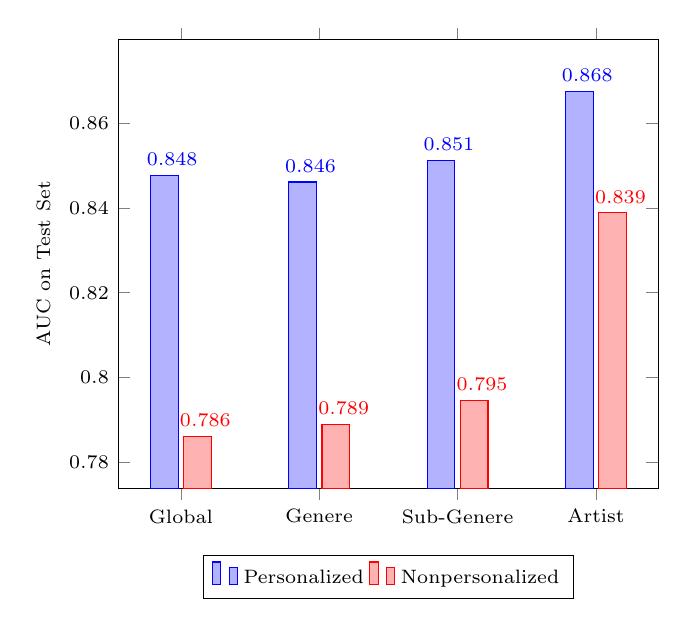
\begin{tikzpicture} 
\begin{axis}[ ybar, enlargelimits=0.15, legend style={at={(0.5,-0.15)}, anchor=north,legend columns=-1}, 
/pgf/number format/precision=3,
font=\scriptsize,
ylabel={AUC on Test Set}, 
symbolic x coords={Global,Genere,Sub-Genere,Artist}, 
xtick=data, nodes near coords, nodes near coords align={vertical},
every node near coord/.append style={xshift=0.1cm}  
 ]
% \addplot[pattern=crosshatch,pattern color=blue]
\addplot   coordinates {(Global,0.847712777) (Genere,0.846150903	) (Sub-Genere,0.851292881)(Artist,0.867522546)};
% \addplot[pattern=north east lines,pattern color=red ] coordinates {(Global,
 \addplot coordinates {(Global,
0.786095642) (Genere,0.788843283) (Sub-Genere,0.794526999)(Artist,0.838879171)};
  \legend{Personalized,Nonpersonalized}
   \end{axis}
    \end{tikzpicture}}    
\subfigure[Groove Music]
{
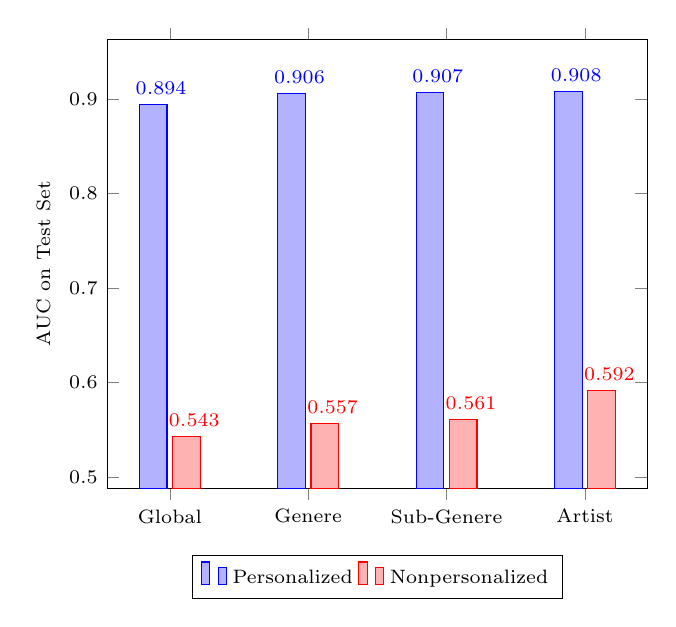
\begin{tikzpicture} 
\begin{axis}[ ybar, enlargelimits=0.15, legend style={at={(0.5,-0.15)}, anchor=north,legend columns=-1}, 
/pgf/number format/precision=5,
font=\scriptsize,
ylabel={AUC on Test Set}, 
symbolic x coords={Global,Genere,Sub-Genere,Artist}, 
xtick=data, nodes near coords, nodes near coords align={vertical},
every node near coord/.append style={xshift=0.1cm}  
 ]
% \addplot[pattern=crosshatch,pattern color=blue]
  \addplot coordinates {(Global,0.894) (Genere,0.906) (Sub-Genere,0.907)(Artist,0.908)};
 %\addplot[pattern=north east lines,pattern color=red ] 
  \addplot coordinates {(Global,0.543) (Genere,0.557) (Sub-Genere,0.561)(Artist,0.592)} ;
  \legend{Personalized,Nonpersonalized}
   \end{axis}
    \end{tikzpicture}

    }
    \caption{The effects of personalization and hierarchy on accuracy are illustrated for (a) the 30Music Dataset (b) the Groove databset}
    \label{fig:MainResultsFig}
 \end{figure}